\section{Introduction}

Atomic chains are a prototype for the study of
molecular electronic systems. Atomic nanowires can be fabricated on
inert surfaces \cite{segovia1999nature,nilius2002science} or in
mechanically controlled break junctions \cite{vanruitenbeek1998mcbj}.
Atomic nanowires are of fundamental scientific interest as they form
electronic one-dimensional systems and for technology they may be viewed
as the limit for metal interconnects in use for nanoelectronics.  Atomic
nanowires are also useful for benchmarking one-dimensional quantum
transport formulations as experiments for these systems provide well
defined and understood conductance values.

Some of the earliest theoretical work with explicit treatment of the
electronic structure within a quatum transport study of atomic chains is
due to Lang~\cite{Lang1995prb}, serving as the model for subsequent
studies in molecular tunnel junctions. In this early work, jellium
electrodes are coupled to metal atom chains and the electronic structure
of the system is treated using \ac{DFT}. The Kohn-Sham states in the
\ac{LDA} approximation are treated as quasiparticles and the electron
scattering equations are solved for the case of an external voltage bias
applied to the electrodes. Similar scattering approaches in conjunction
with tight binding Hamiltonians applied to the conductance of molecular
junctions combined with Landauer-B\"uttiker theory for electron transport
\cite{emberlykirczenow1999standingwave,
emberlykirczenow2000molecularwire} have been undertaken. 
Subsequently, similar methods became commonly used by combining a 
\ac{DFT} treatment of the electronic structure with a formal \ac{NEGF}
treatment of transport in open systems. More recently, the {\it GW}
approximation~\cite{hedin1965gw} has been used to improve  the
quaisparticle description of atomic scale tunnel junctions beyond a Kohn-Sham
description~\cite{thygesen_rubio,neaton2007amines}.  Use of the
Kohn-Sham energies in the NEGF formulation implies a single determinant
or quasiparticle approximation to the many-electron Green's function,
and similarly the {\it GW} approximation may be viewed as a dynamically
screened version of the Hartree-Fock theory, likewise implying a
quasiparticle description. Alternative to these methods are to use the
ideas of exact diagonalization or configuration interaction in rate
equation formulations of electron
transport~\cite{pedersen_many_body_tunneling}, or through a many-electron
scattering formulation of the transport problem~\cite{vici2004,greer2011}. 

In the following, we apply the method of \ac{CI} to a simple model of
electrodes coupled to an atomic chain to investigate the influence of
electron correlations on quasiparticle states arising from the device
region. We explicitly consider the influence of electrode excitations as
they couple to the device region. Opening of the system by the extended
electrodes is modeled by a \ac{CAP} which has been constructed specifically
to yield the same complex energy eigenvaules as a conventional electrode
self-energy would produce~\cite{henderson}. This approach enables us to study
the junction in an uncorrelated limit (single determinant approximation), and
to systematically include electron correlations on the device region and
electrodes to study how the quasiparticle states evolve. 

\section{Methods}
\label{sec:method}

\subsection{Model System}
\label{subsec:modelsystem}

The extended device we study is built from a simple atomic chain
consisting of 68 gold atoms with an interatomic separation of 0.28 nm
approximating the geometry of gold chains studied experimentally in
ref.~\cite{nilius2002science} (see figure~\ref{fig:chaincapdevice}).
Within the explicit chain region, two interatomic spacings are chosen
larger than all other atomic spacings to define a `molecule' between two
leads. The explicit left and right leads are each composed of 24 atoms,
and the central molecular region contains 20 atoms. The width of the gap
between the leads and molecule determines the strength of the
molecule-electrode coupling; varying the spacing allows different
coupling regimes to be investigated. 

The gold atoms are described by a single 6$s$ electron and a 68-electron
effective core potential~\cite{CRENBS} yielding a single half filled
one-dimensional band. The Fock and overlap matrices in the Hartree-Fock
approximation are calculated  using the TURBOMOLE~\cite{turbomole} program
package, and these matrices are used to calculate electron transmission
in the absence of electron correlations with the TiMeS  program~\cite{times}.
The one- and two-electron integrals from the Hartree-Fock calculations
are generated using a modified version of TURBOMOLE and then used to
construct the Hamiltonian matrix elements for the CI calculations.

\begin{figure}
	\begin{center}
		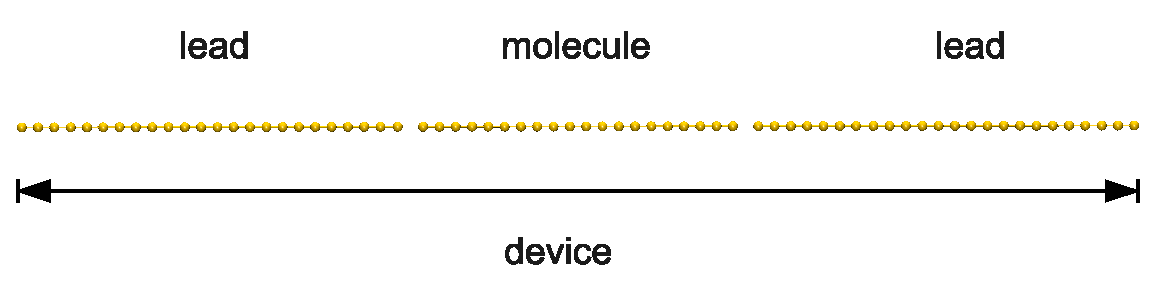
\includegraphics[width=0.9\linewidth]{figures/figure1}
	\end{center}
	\caption{Model system studied in this work. The molecule consists of
        20 Gold atoms, while the explicit electrode regions each consist of 24
	atoms. The spacing between molecules and electrodes determines the
	coupling of the molecular states to the electrodes.}
	\label{fig:chaincapdevice}
\end{figure}

\subsection{Complex Absorbing Potential}
\label{subsec:CAP}

In defining models for atomic-scale transport junctions, a partitioning
of the system into semi-infinite electrodes and device region is typically
performed. The device region is given by an explicit model that includes
the device (i.e. atomic chain, molecule, nanowire) as well as a region
that defines the bonding of the device to electrodes, resulting in an
`extended device' or `extended molecule'. The portion of the
electrode not explicitly treated by the extended device region in
most theoretical studies is then treated by electrode self-energies. In this
approximation, electronic excitations in the electrode region are not
considered. Exceptions include ref.~\cite{galperin_nitzan2006leadexcitations}
where the effect of coupling of lead excitations to a two state model of
a molecular tunnel junction is explored, and a recent formulation
of \ac{NEGF} that allows for electrode interactions to be explicitly
treated~\cite{ness2012jpa_leadnegf}. However with this approach, excitations
from the electrode portions that are explicitly included in the explicit
device region can be included if the electronic structure treatment of
the device regions allows for electron correlations.

In this study, the regions outside of the explicit atomic region are
described by a \ac{CAP} in analogy to the use of electrode self-energies.
The details of the \ai \ac{CAP} used are described below and its use has
advantages when including electron correlations into the calculations.
As our leading or 0$^{th}$ order approximation, we use the Hartree-Fock
orbitals to calculate the transmission spectrum for the model system using
a Green's function approach  as implemented in the TiMeS program~\cite{times};
the electrodes in these (uncorrelated) scattering calculations are
described using standard electrode  self-energies. This scattering
calculation delivers the Hartree-Fock quasiparticle spectrum including
the energy shifts and state broadening that arise from coupling the molecular
region to electrodes, and serves as the reference point for discussing
subsequent calculations performed as we introduce correlations into the
calculations. 

To treat electron correlations, we apply the method of \ac{CI}. The \ac{CI}
method is the application of the  Rayleigh-Ritz linear variational
principle to the calculation of quantum many-electron  energies. Within
this approach, the many-electron wavefunction is expanded in terms  of
Slater determinants (or spin-coupled sums of determinants referred to as
\acp{CSF}).  Variation of the \ac{CI} expansion coefficients leads to a
matrix eigenvalue problem
\begin{equation}
\um{H} \vec{c} = E \um{S} \vec{c},
\end{equation} 
where $\um{H}$ is the matrix representation of the many-electron
Hamiltonian in the CSF basis, $\um{S}$ is the metric for the CSF basis,
$E$ is a many-electron energy and $\vec{c}$ is the vector of the
expansion coefficients or CI vector. The matrix elements of $\um{H}$
and $\um{S}$ are constructed from one- and two-electron integrals
defined in the single particle basis used to construct the CSFs, and for
example can be Hartree-Fock states. However, in the CI treatment of the
many-electron problem, no reference is made to single particle or
quasiparticle energies. Hence the inclusion of the electrodes into the
CI problem using electrode self-energies is complicated by the fact that
the self-energies are functions of the quasiparticle energies on the
electrodes. To avoid this complication, we employ instead energy-independent
\acp{CAP} that serve as replacement to the self-energy terms, eliminating
reference to single particle energies into the resulting \ac{CI}
problem~\cite{riss_meyer,santracederbaum,muga2004,henderson,varga2008}.
Note however, that by opening the system using either electrode self-energies
or \acp{CAP},  the traditionally Hermitian \ac{CI} generalized eigenvalue
problem becomes a complex symmetric generalized eigenvalue problem. The
procedure we follow for construction of an energy-independent \ai \ac{CAP} 
from the energy-dependant self-energy is discussed in detail
in~\cite{henderson}, and we briefly cover the essential points needed
for the generation of the \ac{CAP} in the following.

We first consider a system with bare Hamiltonian $\um{H}_0$ in the
Hartree-Fock approximation, coupled to two electrodes described by known
left $\um{\Sigma}_L(\omega)$ and right $\um{\Sigma}_R(\omega)$ self-energies.
These self-energies are added to the single particle
Hamiltonian to yield
\begin{eqnarray}
\label{eq:capseq}
        [\um{H}_0 + \lambda \um{\Sigma_L}(\omega_i^\lambda)
            +\lambda \um{\Sigma_R}(\omega_i^\lambda)] \ket{U_i^\lambda}
        &= \omega_i^\lambda \ket{U_i^\lambda} \\
        \bra{V_i^\lambda} [\um{H}_0 + \lambda \um{\Sigma_L}(\omega_i^\lambda)
            +\lambda \um{\Sigma_R}(\omega_i^\lambda)]
        &= \omega_i^\lambda \bra{V_i^\lambda},
        \label{eq:adiabaticap}
\end{eqnarray}
where the parameter $\lambda$ is introduced to allow for an adiabatic
transition between eigenstates $\ket{X_i}$ of $\um{H}_0$ at $\lambda = 0$,
and the true, finite-lifetime resonant states of the system at
$\lambda = 1$. The Hartree-Fock states for the open system are given by
the complex energies $\omega_i$, right eigenvectors $\ket{U_i}$ and left
eigenvectors $\bra{V_i}$; distinct left and right eigenvectors are a
consequence of introducing the complex symmetric self-energy matrices into
the eigenvalue problem.
The adiabatic introduction of the self-energies permits
us to `label' the molecular states and to follow their evolution as the
system is opened. This allows us to select those eigenstates (and
eigenvalues) of the coupled system that correspond to states of the
uncoupled device region. At $\lambda=1$, the real part of $\omega_i$
gives the energy of the $i$th resonance including the shift due to
electrode coupling and the imaginary part gives the level broadening.

The goal is to build an energy-independent complex potential
$\um{W} = \um{W_L} + \um{W_R}$
such that the Hamiltonian $\um{H}_0 + \um{W}$ has the same eigenvalues
as when calculated using the explict self-energies. Such a Hamiltonian is
not readily constructed as when we select the different $\omega_i$, we are
as a consequence selecting different Hamiltonians
$\um{H}_0 + \um{\Sigma_L}(\omega_i) + \um{\Sigma_R}(\omega_i)$
and the biorthogonality for the left and right eigenvectors does not
necessarily hold ($\bracket{V_i}{U_j} \ne \delta_{ij}$). We consider instead
constructions which yield eigenvalues that approximate the $\omega_i$  and
eigenvectors that approximate the left and right eigenvectors while
satisifying biorthogonality. Given such a set of approximate eigenvectors
we write
\begin{equation}
    \um{W} = \sum_i  \ket{U^\prime_i} \omega_i \bra{V^\prime_i} - \um{H}_0
    \label{eq:capsdefUV}
\end{equation}
which for biorthogonal $\ket{V^\prime_i}$ and $\bra{U^\prime_i}$ will by
construction give an operator $\um{H}_0 + \um{W}$ with the correct eigenvalues
and approximate eigenvectors. In practice we work in the real basis of the
device region and calculate
\begin{equation}
    \um{W} = \um{S} \um{X} \boldsymbol{\omega}\um{X}^\dagger - \um{H}_0
    \label{eq:capsdefX}
\end{equation}
in matrix form, where $\um{S}$ is the overlap or metric for the atomic
orbital basis used to describe the system, $\um{X}$ is the matrix of the
eigenvectors of the Hamiltonian $\um{H}_0$, and $\boldsymbol{\omega}$ is a
diagonal matrix with the eigenvalues $\omega_i$ calculated at
$\lambda = 1$ along the diagonal.
In practice, since the self-energiy is a property of the electrode only
(for properly defined electrodes and device regions), the \acp{CAP} are
generated on a single unit cell of the lead, and then transformed to the
molecular orbital basis of the device region, which contains a lead unit
cell on either side.

A comparison can be performed for this approximation of a \ac{CAP} 
against the energy level shifts and broadening
obtained from explicit calculations using the self-energy. To accomplish
this comparison, we first calculate the electron transmission through
the device region using the Green's function
approach. The calculation is then repeated but in the definition of the
Green's function ${\bf G}$ and spectral densities ${\bf \Lambda}_{L/R}$ the
self-energy terms are replaced with the \acp{CAP} $\um{W}_{L/R}$ leading
to the following expressions:
\begin{eqnarray}
	  \um{G}^{-1} &= [E\um{S} - (\um{H}_D + \um{W})], \\
	  \um{\Lambda}_{(L/R)} &= i \left( \um{W}_{(L/R)} - \um{W}^\dagger_{(L/R)}
    \right).
  \label{eq:glambdadef}
\end{eqnarray}
($\um{H}_D$ is the Hamiltonian of the extended device region.) The
transmission is then calculated as
\begin{equation}
  T = \um{Tr} \left[ \um{\Lambda}_L \um{G} \um{\Lambda}_R \um{G}^\dagger \right]
  \label{eq:transmfromG}
\end{equation}
where the \acp{CAP} play the role of the electrode self-energies.
The comparison obtained in this manner is shown in fig.~\ref{fig:transdat}
revealing that the \ac{CAP} provides an accurate energy-independent
representation of the self-energies and in particular, excellent agreement
is achieved on the energy range around the \ac{HOMO}-\ac{LUMO} gap of
interest which is the focus of our subsequent calculations.

\begin{figure} 
	\begin{center}
		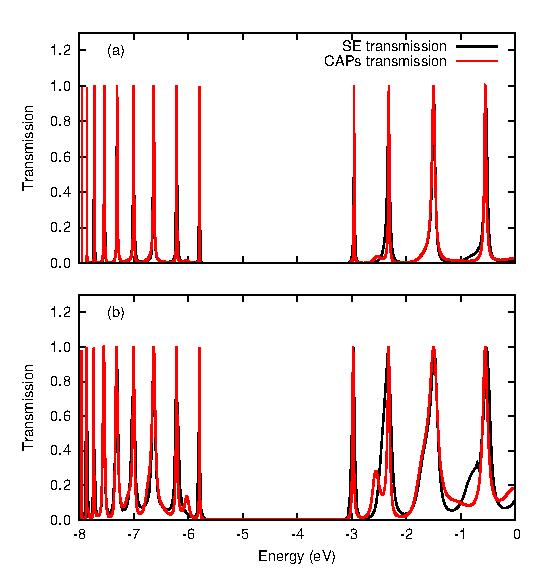
\includegraphics[width=0.9\linewidth]{figures/figure2a_2b}
	\end{center}
	\caption{Transmission through the chain junctions obtained in
	         scattering calculations with a Green's functions formalism
		 and with lead-molecule separations of 0.45 nm (top) and 0.40
		 nm (bottom). The red curve is a transmission spectrum obtained
		 using a conventional self-energy, the green curve is
		 obtained using a \ac{CAP}.}
	\label{fig:transdat}
\end{figure}

Having verified that the \acp{CAP} are able to reproduce the electron
transmission to a good approximation compared against using explicit
electrode self-energies, we next examine if the transmission resonances
can be well approximated as Lorenztian resonances. This question is
motivated by the fact that in our subsequent many-body treatment,
quasiparticle energies will be calculated as differences of complex
many-electron state energies. If we may approximate the transmission
resonances as Lorentzian peaks, then the complex quasiparticle energies 
can be used to generate Lorentzian transmisson functions for direct
comparison to the scattering function transmissions (there is some
indication of Fano-type resonances indicating that there is a degree of
coupling between electrodes, but these small effects do not influence
our analysis). To investigate this point, Lorentzian  resonances are
constructed using the complex eigenvalues $\omega_i$ obtained from the 
\acp{CAP} eq.~\ref{eq:capseq} with $\lambda=1$, 
\begin{equation}
        f(\varepsilon;\omega_i)
        = \frac{\left( \Gamma/2 \right)^2}
               {(\varepsilon - \mathrm{Re}(\omega_i))^2
               + \left( \Gamma/2 \right)^2},
        \label{eq:lobro}
\end{equation}
where $\Gamma = 2 \mathrm{Im}(\omega_i)$ (i.e., the width of the
Lorentzian peak) and is inversely proportional to the lifetime of the
quasiparticle. These Lorentzian resonances are compared to the transmission
spectrum of the device obtained using explicit self-energies and a
scattering calculation; the results of the comparison are shown in
fig.~\ref{fig:13evals} for the chain system with molecule-lead separation
of 0.45 nm (weak coupling case). The Green's function transmission and
the peaks derived from the complex eigenvalues of $\um{H}_D + \um{W}$
(green) agree extremely well, both in terms of the energy of the transmission
peak (real part) and resonance width (imaginary part).  The inset in
fig.~\ref{fig:13evals} displays the region around the \ac{HOMO} in
detail, and reveals that the transmission peaks are well described by a
Lorentzian profile and that the CAPs are able to reproduce quasiparticles
within an accuracy required for our study.

\begin{figure} 
	\begin{center}
		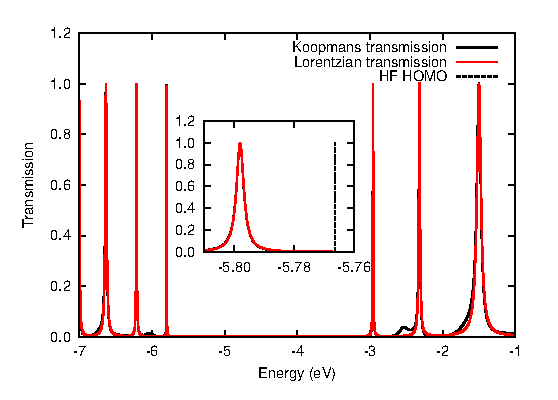
\includegraphics[width=0.9\linewidth]{figures/figure3}
	\end{center}
	\caption{Comparison of transmission data obtained using a self-energy
	(red) with Lorentzian broadened complex eigenvalues of $\um{H}_D + \um{W}$
	(green) for a model system as described in
	section~\ref{subsec:modelsystem}, with device-lead gap of 0.45 nm.
	The inset shows a close-up view of the \ac{HOMO}, with the HF \ac{HOMO}
	shown in blue for reference.
	}
	\label{fig:13evals}
\end{figure}

\subsection{Complex Symmetric \ac{CI} Problem}

All \ac{CI} calculations  are performed using a version of the \ac{MCCI}
program~\cite{mcci1995, mcci1998} modified to treat the complex
symmetric generalized eigenvalue problem that arises when adding the
\ac{CAP} to the many-electron Coulomb Hamiltonian. The \ac{CAP} is
introduced as a one-body operator describing the extended device region 
and its interaction with the elecrodes into the \ac{CI} Hamiltonian. 
\ac{MCCI} uses a modified Lanczos method for matrix diagonalization and
in the complex symetric version of the program, the projection method
outlined in~\cite{tarantelli_csd} is introduced to solve the complex
symmetric generalized eigenvalue problem. 

\ac{MCCI} computes energy estimates by an iterative process, starting from
a set of \acp{CSF} (which initially may be a single \ac{CSF}). In each step,
additional \acp{CSF} are randomly generated by single and double excitations
relative to the \acp{CSF} in the trial vector. The \ac{CI} matrix
diagonalization problem is solved on the subspace defined by the resulting
expanded vector. This vector is then screened or `pruned' by removing
\acp{CSF} whose associated coefficient in the \ac{CI} eigenvector has a
magnitude lower than a given threshold. This pruned vector serves as
trial vector for the generation of a new set of randomly generated
\acp{CSF}s in a subsequent cycle, and  this sequence is repeated until
convergence in the energy and CI vector length is reached. Details of the
\ac{MCCI} method may be found in 
refs.~\cite{mcci1995,mcci1998,mcci2000,multiref}.

The use of \ac{MCCI} in the present study allows us to follow the
evolution of quasiparticle energies as electron correlations are
increased; this is achieved by starting from a single determinant picture
and then systematically including important electron correlations by
performing \ac{CI} calculations at different values of the coefficient
selection threshold. As the coefficient selection threshold is reduced,
more \acp{CSF} are included in the calculations leading to improving
descriptions of electron correlations.

\subsection{CI approximations}

In our analysis, we consider several different approximations for the CI
wavefunction expansions. The first set of approximations are derived from
CI expansions consisting of single excitations 
\begin{equation}
\label{singles}
  \ket{\Psi_0} + \ket{\Psi_{S}}
  =
  \left(1 + \sum_{i,a} c_i^a \hat{a}_a^\dagger \hat{a}_i \right) \ket{\Psi_0},
\end{equation} 
with $\ket{\Psi_0}$ the Hartree-Fock reference state, $\ket{\Psi_{S}}$
consists of the singly excited CSFs, $i$ is an index over occupied
orbitals, $a$ is an index over unoccupied states, $c_i^a$ is the CI
coefficient for a singly excited CSF, and $\hat{a}^\dagger$ and $\hat{a}$
are creation and annihilation operators, respectively. The use of this
form of the CI wavefunction allows for the investigation of the effect
of optimizing the single particle orbitals. This may be understood by
considering Thouless' theorem~\cite{thouless} which relates two arbitrary
determinants $\ket{\Psi_A}$ and $\ket{\Psi_B}$ through  an exponential
operator as
\begin{equation}
\label{thouless}
\ket{\Psi_A} = \exp \left( \sum_{i,a} c_i^a a_a^\dagger a_i \right) \ket{\Psi_B}.
\end{equation}    
The exponential operator acts as a rotation to the single particle basis.
For appropriately selected coefficients $c_i^a$, $\ket{\Psi_A}$ can be
chosen as the single particle determinant which optimizes, for example,
the energy on the extended device region. If the reference weight of
$\ket{\Psi_0}$ in the singles wavefunction is large, then the expansion
coefficients $c_i^a$ will be small and eq.~\ref{singles} becomes an
approximation to the Thouless form eq.~(\ref{thouless}), accurate to first
order in the $c_i^a$. 

From a many-electron standpoint, energy differences between many-electron
states determine quasiparticle excitations, as well as electron affinities
and ionization energies, or respectively addition and substraction energies. 
In this study, the focus is on the electron affinities and ionization
potentials of the {\it explicit} device region as these can be directly
related to the quality of an electronic structure description for transport
calculations~\cite{golden}. For example, the electron affinity is given
by the difference in energies for the $N$-electron state $E^N$ and the
$(N+1)$-electron state $E^{N+1}$
\begin{equation}
\label{eq:EA}
\omega_{\rm EA} = E^{N+1} -E^N,
\end{equation}
and similarly the ionization potential
\begin{equation}
\label{eq:IP}
\omega_{\rm IP} =  E^N - E^{N-1}
\end{equation}
is the energy difference between the $(N-1)$- and $(N)$-electron states.
The inclusion of the set of singly excited configurations allows a
comparison on the explicit device region between a Koopmans approximation 
(no orbital relaxation) and a \dscf approximation (inclusion of
orbital relaxations).  For example, in the transmission displayed in
fig.~\ref{fig:transdat}, the resonances correpsond to the eigenvalues of
the $N$ particle Fock matrix that are shifted in energy and broadened due
to the inclusion of the electrode self-energies. Hence the \ac{HOMO} state
corresponds to the IP for the extended device region but excluding the
effects of relaxation of the other single electron states that occurs
when an electron is removed. Likewise the LUMO measures the energy gained
by attaching an electron onto the device region with all other electrons
frozen. In this sense, the resonances are identified as Koopmans' IP and
EA. If the IP and EA are calculated from a many-electron viewpoint and
with the inclusion of the single excitations into the CI wavefunction,
all other electrons can relax on the extended device region as the charge
state is changed. As Thouless' theorem tells us that the CI singles
energies $E^{N-1}$ and $E^{N+1}$ are approximations to the optimized
single determinant energies with orbital relaxations for the device region,
the EAs and IPs eqs.~\ref{eq:EA} and \ref{eq:IP} correspond to a \dscf
approximation. 

Two types of CI singles approximations are considered. The first set are
referred to as molecular singles, in these calculations only one-electron
or singles excitations to and from orbitals derived from the molecular
region are allowed. In the second set of singles, all orbitals on the
extended device region whether arising from the molecular or the explicit
electrode regions are allowed. This latter approximation is referred to
as the device singles. The CI singles as discussed remain a single
particle description of the tunnel junction. To include correlations,
MCCI calculations with coefficient thresholds of 0.003 and 0.001 are
performed. Again, two such sets of calculations are performed. In the
first set, only excitations to and from the molecular derived states are
allowed and are retained in the MCCI procedure based upon the value of
the coefficient threshold. These CSFs are labelled as CI(0.003) molecule
and CI(0.001) molecule. For the extended device region, a single MCCI
calculation is performed with a coefficient cut-off of 0.003 with
excitations to and from all orbitals permitted. This set of CSFs is
labelled CI(0.003) device. 

\section{Quasiparticle States and Lifetimes}

Through the introduction of the \acp{CAP} describing the electrodes, the
device region becomes an open system resulting in complex many-electron
energies. Hence the quasiparticle energies $\omega_i$, calculated  as the
difference in energies between many-electron states, are also complex
valued. It is the energy shift (related to the real part of $\omega_i$)
and finite lifetime (related to the imaginary part of $\omega_i$) due to
the opening of the system and as electron correlations are introduced on
the extended device region which we study for quasiparticles on the
tunnel junction.

We start our analysis by considering the model with weaker coupling
defined by a 0.45 nm gap between the electrodes and molecular region,
and initially only including electronic excitations for orbitals localized
on the molecular region. As can be seen in fig.~\ref{fig:13evals}, the
main effect of the electrode coupling at the single particle level is an
energy shift in the HOMO level of 32 meV and a state broadening indicating
a lifetime $\tau$ of approximately 223 fs, as calculated by
$\tau = \hbar / \Gamma$.

Performing a molecular singles calculation with only molecule orbital
excitations, we see the HOMO peak shifts upward in energy by 288 meV and
the LUMO peak shifts downward in energy by 260 meV as seen in the blue
curves within figs.~\ref{fig:all45Ahomo} and \ref{fig:all45Alumo}, hence
the overestimation of the bandgap typical of the Hartree-Fock approximation
is compensated for this approximate \dscf calculation.
The electron lifetimes decrease substantially relative to the Koopmans
states with the HOMO state lifetime becoming 59 fs and the LUMO state
becoming 17 fs when self-consistency is allowed, indicating an increased
molecule-electrode coupling. 
Introducing electron correlations using using the molecule-like orbital
set and a coefficient threshold of 0.003 in the MCCI calculations lowers
the molecular HOMO and increases the energy of the LUMO. Further increasing
the correlation allowed with use of a MCCI coefficient threshold of 0.001,
but still only using molecule-like excitations, further reduces the energy
of HOMO resonance and slightly lowers the resonance peak of the LUMO.
These findings for the weakly coupled molecular state are consistent with
typical findings for molecular systems: the Koopmans EAs and IPs are 
underestimated and overestimated, respectively, whereas the \dscf
procedure tends to overestimate and underestimate EAs and IPs, respectively.
Introducing electron correlations then renormalizes the funamental gap
with the correlated energies for the HOMO and LUMO states bracketed by
the Koopmans and \dscf estimates.
Hence in the weakly coupled case and including only excitations to and
from molecule-like orbitals, we find that the molecular region behaves
very much like an isolated molecule, with the additional features of an
energy shift and a finite state lifetime due to the molecule-electrode
coupling.
Introducing self-consistency into the model shifts and signiciantly
broadens the resonance peaks as shown in figs.~\ref{fig:all45Ahomo} and
\ref{fig:all45Alumo}.
Improving the approximation to the quasiparticle states by allowing an
increased description of electron correlations introduces significant
energy shifts to the resonance peaks but is found not to substantially
change the broadening relative to the \dscf resonances.

Next, the effect of stronger coupling is considered by reducing the gap
between the electrodes and molecular regions to 0.40 nm.
A similar behavor is seen as compared to the weaker coupling case. The
\dscf approximation again shifts the energies of the HOMO and LUMO
resonances reducing the energy gap, and the state broadening relative to
the Koopmans resonances is significantly altered with state lifetimes
decreasing to approximately 17 fs from 71 fs, and to 7 fs from 26 fs for
the HOMO and LUMO, respectively.
Again it is found that increasing correlation shifts the energies of the
resonances but does not significantly alter the lifetime broadening beyond
that introduced at the \dscf level. Introducing electron correlations
again renormalizes the energy gap, with the correlated resonant states
bracketed by the Koopmans and \dscf values.

\begin{figure}
	\begin{center}
		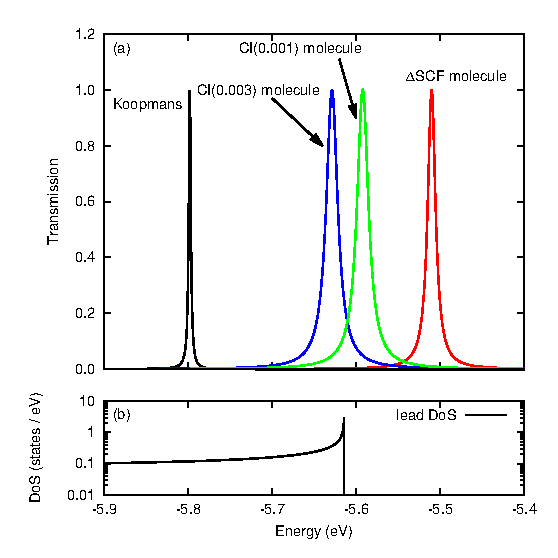
\includegraphics[width=0.9\linewidth]{figures/figure4a_4b}
	\end{center}
	\caption{HOMO region quasiparticle peaks of the 0.45 nm separated
	         system, with excitations restricted to the `molecule' region,
		 at different levels of theory: HF + self-energy (red),
		 \dscf (green), and MCCI with threshold parameters of
		 0.003 (blue) and 0.001 (magenta).}
	\label{fig:all45Ahomo}
\end{figure}

\begin{figure}
	\begin{center}
		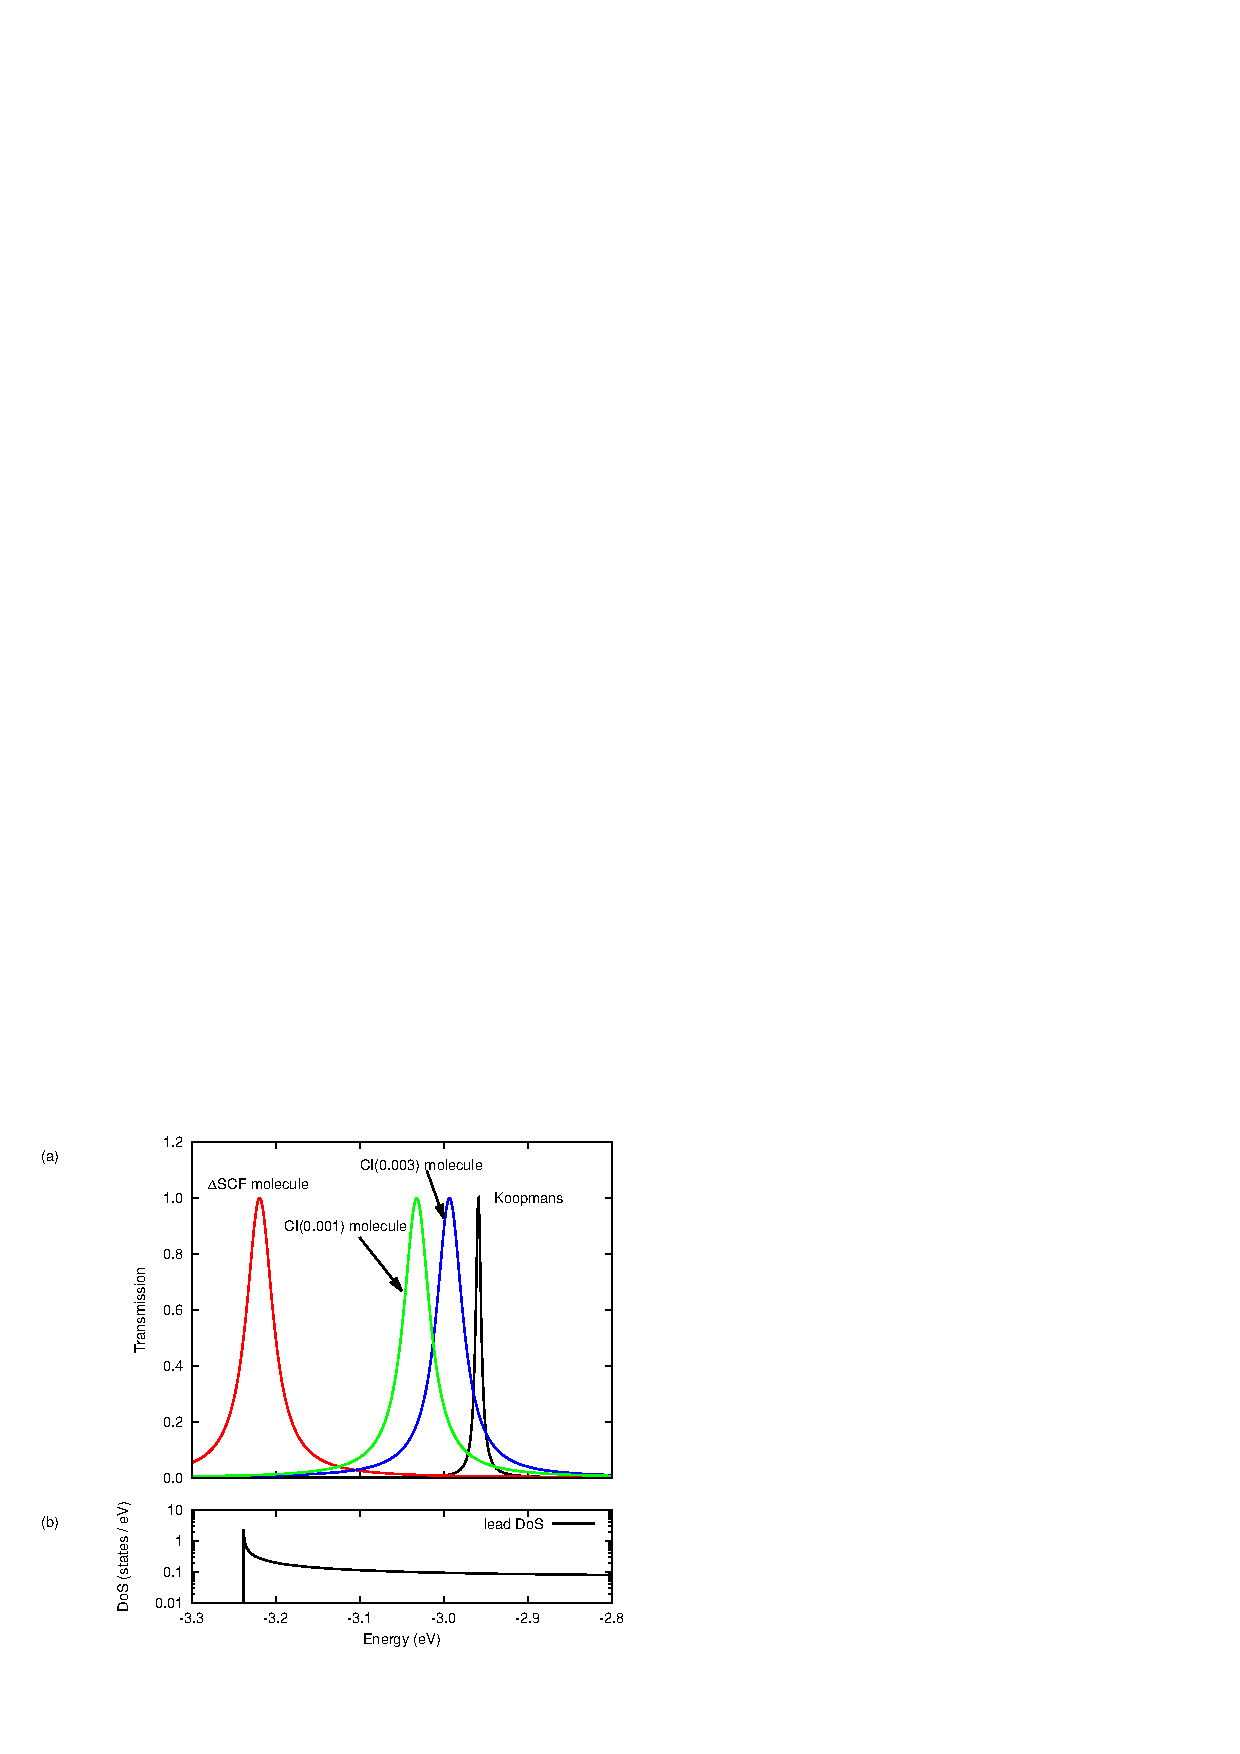
\includegraphics[width=0.9\linewidth]{figures/figure5a_5b}
	\end{center}
	\caption{LUMO region quasiparticle peaks of the 0.45 nm separated
	         system, with excitations restricted to the `molecule' region,
		 at different levels of theory: HF + self-energy (red),
		 \dscf (green), and MCCI with threshold parameters of
		 0.003 (blue) and 0.001 (magenta).}
	\label{fig:all45Alumo}
\end{figure}

\begin{figure}
	\begin{center}
		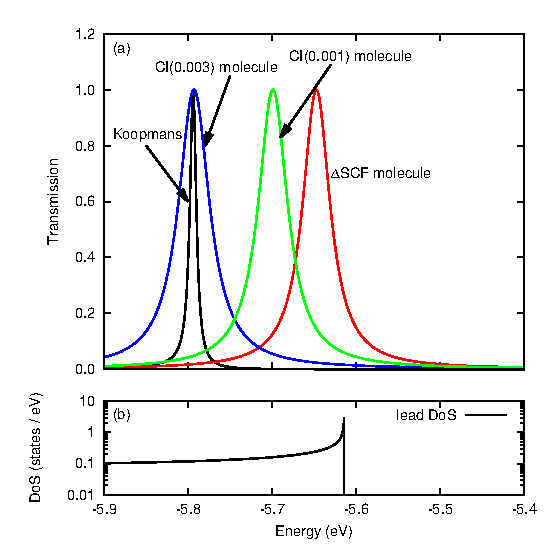
\includegraphics[width=0.9\linewidth]{figures/figure6a_6b}
	\end{center}
	\caption{HOMO region quasiparticle peaks of the 0.40 nm separated
	         system, with excitations restricted to the `molecule' region,
		 at different levels of theory: HF + self-energy (red),
		 \dscf (green), and MCCI with threshold parameters of
		 0.003 (blue) and 0.001 (magenta).}
	\label{fig:all40Ahomo}
\end{figure}

\begin{figure}
	\begin{center}
		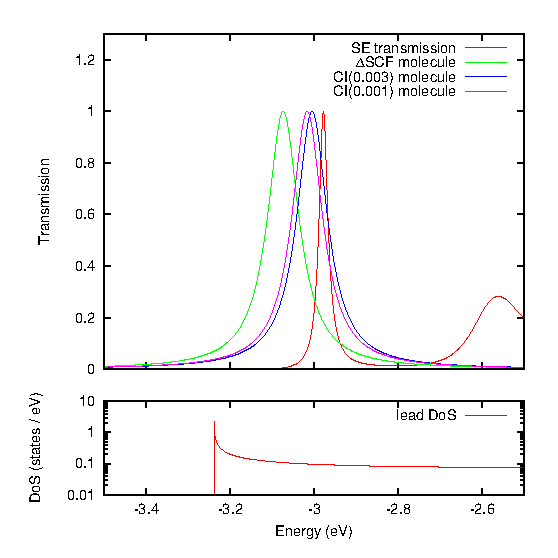
\includegraphics[width=0.9\linewidth]{figures/figure7a_7b}
	\end{center}
	\caption{LUMO region quasiparticle peaks of the 0.40 nm separated
	         system, with excitations restricted to the `molecule' region,
		 at different levels of theory: HF + self-energy (red),
		 \dscf (green), and MCCI with threshold parameters of
		 0.003 (blue) and 0.001 (magenta).}
	\label{fig:all40Alumo}
\end{figure}

Finally, we investigate the effect of including excitations from the
explicit electrode region included within the definition of the extended
device region. Until this point, we have constrained the CI space to only
\acp{CSF} including excitations from and to orbitals localized on the
molecular region. However, in a previous work it has been shown that the
coupling of electrode exciations to the molecular excitations can have
significant effects on current flow through a correlated two-level model
system~\cite{galperin_nitzan2006leadexcitations}. 

We study again the more weakly coupled model defined by a 0.45 nm gap
between the electrodes and the molecular region, this time allowing
excitations that are molecule-like as well as ones relating to orbitals
from the explicit electrodes to enter the calculations;
the results are displayed in the top pane of \fref{fig:cidevregion}. 
Since self-consistency is introduced by approximating Thouless' theorem
with all single excitiations on the extended device region, the energy gap
between HOMO and LUMO narrows with respect to the Koopmans values, as
previously was the case. However, in this case the \dscf results
in much larger energy shifts with respect to a \dscf approximation
relying on excitations from only molecule-like orbitals. There is also a
significant difference in the resonant broadening, the HOMO state lifetime
decreases from the Koopmans estimate of 223 fs to 18 fs as obtained from
the \dscf approximation. 
However, much less resonant broadening is seen in this example for the
LUMO state, with a lifetime of 85 fs from the HF + self-energy approximation
and 121 fs from the $\Delta$SF calculation. The results of introducing
correlation with a MCCI vector generated with a coefficient threshold of
0.003 is seen in the blue curve of \fref{fig:cidevregion} and again a
renormalization of the energy gap is seen.
{\bf I thought renormalization always meant a narrowing of the gap?}
However, as electrode excitations are allowed to couple to the
molecule-like excitations, the correlated HOMO and LUMO resonance energies
are no longer bracketed by the HF + self-energy and \dscf peaks.
There is also a difference in the behavior for the HOMO and LUMO resonances.
For the HOMO peak, the lifetime stays approximately the same as in the
$Delta$SCF approximation whereas electron correlations broaden the LUMO
peak from a lifetime of 121 fs from the \dscf approximation to 21
fs. 

As the electrode-molecule distance is reduced to 0.40 nm, the increased
coupling in combination with the inclusion of electrode excitations
introduces quantitatively and qualitatively different behavior compared
to all previous cases we have studied. Including the electrode interactions
with the \dscf approximation as for the 0.45 nm coupling case,
significantly reduces the QP gap and the magnitude of the correction to
the gap energy for the 0.40 and 0.45 nm cases are similar. For the state
lifetimes, the HOMO state is approximately the same as for the 0.45 nm
case, whereas the LUMO state is significantly broader than all calculations
previously presented with a lifetime of $\approx 2$ fs. In this case,
the CI singles approximation to the $N+1$-electron state becomes
multi-reference with two CSFs predominately contributing in the expansion.
One of these CSFs has the additional electron in an electrode orbital,
whereas the other consists of an additional electron into the molecule's
LUMO. Hence in \dscf approximation to the LUMO, the electrodes and
molecule regions are strongly coupled leading to a broad resonance.
Introducing electron correlations with the MCCI vector obtained from a
coefficient threshold of 0.003 leads to further anomalous behavior. The
QP gap is again renormalized by the electron correlations, however in the
case the HOMO state remains approximately unchanged although there is
slightly more broadening and a small energy shift. However the character
of the LUMO state relative to the \dscf approximation changes: the
electron correlations help to decouple the state from the electrodes
resulting in a single dominant CSF in the CI expansion that describes the
added electron as a molecule-like state. The energy broadening decreases,
leading to a lifetime of $\approx 7$ fs, and the state has shifted upward
by approximately 1 eV.
 
\begin{figure}
	\begin{center}
		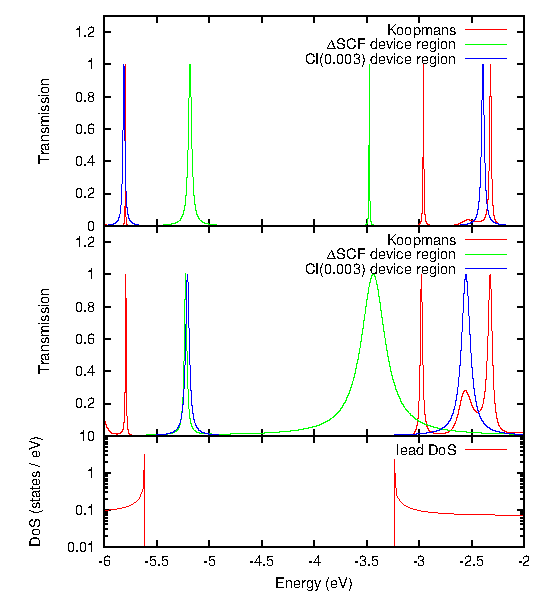
\includegraphics[width=0.9\linewidth]{figures/figure8a_8c}
	\end{center}
	\caption{CI results with inclusion of lead excitations for the
	         0.45 (top) and 0.40 nm (middle) systems, with the Density
		 of States of the leads plotted below.}
	\label{fig:cidevregion}
\end{figure}

Finally, as an illustration of how the changes in transmission curves would
affect the devices' conductance properties, we calculate the $I-V$ curves
for the 0.40 nm separated junction in the different levels of theory,
using the Landauer-B\"uttiker formalism~\cite{buttiker1986}. In the top
pane of \fref{fig:iv}, we have plotted the results for the \dscf (both
molecule and device region) and Koopmans transmissions. The wide LUMO
peak which was noted earlier for the device region case causes an earlier
onset and higher final value of the current than in the case of the
molecule. The Koopmans curve has a later onset, due to the higher bandgap,
but at higher voltages the current exceeds that of the \dscf cases, since
it contains more than just the HOMO and LUMO levels. The current from
the Koopmans transmission including only the HOMO and LUMO levels is
plotted in \fref{fig:iv}. The lower pane shows the current from the two CI
transmissions. Due to the peaks in both cases being roughly the same
width, the current reaches similar values for high voltages, but the
higher position of both `device region' peaks relative to their `molecule'
counterparts causes a different onset behavior.

\begin{figure}
	\begin{center}
		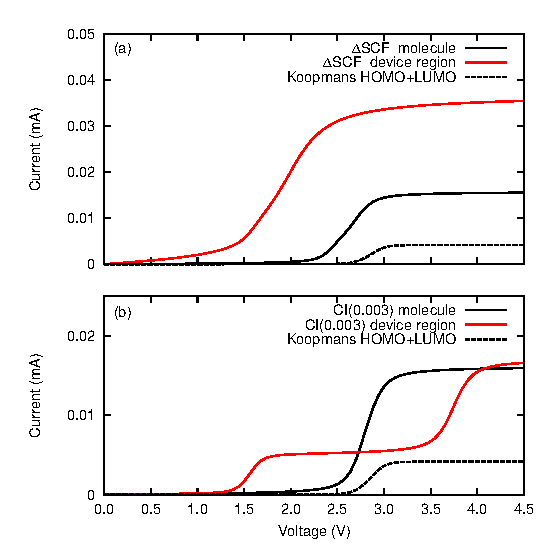
\includegraphics[width=0.9\linewidth]{figures/figure9a_9b}
	\end{center}
	\caption{Current versus voltage for the different transmission
	         spectra discussed above, using the Landauer formula.
		 Note that this is slightly artificial in this case, as
		 the chain leads have a band gap. The equilibrium Fermi
		 energy was chosen to lie in the middle of the band gap
		 of the leads, at $-4.42$ eV, and as voltage is applied
		 the electrochemical potentials on either side are taken
		 to move symmetrically.}
	\label{fig:iv}
\end{figure}
 
\section{Conclusions}
\label{sec:conclusions}

This study has focused on the examination of the electronic structure
treatment of molecular tunnel junctions, and in particular has studied
the impact of the electronic structrure treatment on quasiparticle
energies and lifetimes. A simple model of a tunnel junction was introduced
and consists of an atomic gold chain partitioned into left and right
electrodes, and a central `molecule'. The electrode self-energies were
approximated using complex absorbing potentials (\acp{CAP}) enabling the
use of a configuration interaction method. The use of the \acp{CAP} was
validated against calculations using explicit electrode self-energies.
The junction model was investigated using a non-self consistent single
particle treatment or Koopmans treatment of quasiparticle states, an
approximate self-consistent treatment based on a CI singles expansion,
and including electron correlations within truncated many-body expansions.
Two values of electrode coupling were studied by varying the distance
between the electrode and molecular regions. The ability to predict
electron affinities and ionization potentials was assessed as it has been
shown that the quality of a quantum transport calculation may be directly
related to the ability to predict electronegativity within the electronic
structure description of the junction~\cite{golden}. 

The calculations were further divided into two forms: those that did not
allow electronic excitations from the elecrodes into the CI calculations,
and those that did. In the case that electrode excitations were excluded
from the \dscf and CI calculations, and for the range of electrode
couplings we considered, it was found that the molecule in the junction
behaved analogously to a free molecule. The Koopmans approximation
overestimated the QP energy gap, the \dscf approximation underestimated
the gap, and including explicit electron correlations renormalized the
energy gap with the HOMO and LUMO states being bracketed by the Koopmans
and \dscf estimates. However, these findings are fundamentally
altered when electrode excitations are included consistent with the findings
of~\cite{galperin_nitzan2006leadexcitations}.
The junction's electronic structure becomes less like that of a free
molecule and the QP states and lifetimes are heavily influenced by both
the amount of correlation and the degree of coupling. The impact of the
different electronic structure treatments for the junction is highlighted
current plots of fig.(XX) %~\ref{fig:IVfig}.
